\subsection{Exercise~1.15}

The author has no idea how to prove the desired homeomorphism with using Corollary~2.18.2.
We will therefore use this criterion at some point.

We will consider more generally the disk
\[
	\disk^n = \{ x ∈ ℝ^n \suchthat \norm{x} ≤ 1 \}
\]
and sphere
\[
	\sphere^n = \{ x ∈ ℝ^{n + 1} \suchthat \norm{x} = 1 \} \,.
\]
Let~$∼$ be the equivalence relation on~$\disk^n$ that identifies all boundary points of~$\disk^n$, i.e., all points of~$\sphere^{n - 1}$.
We construct in the following a homeomorphism between~$\disk^n / {∼}$ and~$\sphere^{n - 1}$.
We will proceed as depicted in \cref{construction of disk modulo sphere}.
\begin{figure}
	\[
		\centerbox{
		\begin{tikzpicture}[scale=0.35]
			% axes
			\draw[->,black!50] (-2.5, 0) -- (2.5, 0);
			\draw[->,black!50] (0, -2.5) -- (0, 2.5);
			% disk
			\draw[thick, fill] (-1, 0) -- (1, 0);
			% circles
			\draw[fill] (-1, 0) circle (0.1);
			\draw[fill] ( 1, 0) circle (0.1);
		\end{tikzpicture}
		}
		\quad≅\quad
		\centerbox{
		\begin{tikzpicture}[scale=0.35]
			% axes
			\draw[->,black!50] (-2.5, 0) -- (2.5, 0);
			\draw[->,black!50] (0, -2.5) -- (0, 2.5);
			% hemisphere
			\draw[thick] (-1, 0) arc (180:0:1);
			% end points
			\draw[fill] (-1, 0) circle (0.1);
			\draw[fill] ( 1, 0) circle (0.1);
		\end{tikzpicture}
		}
		\quad≅\quad
		\centerbox{
		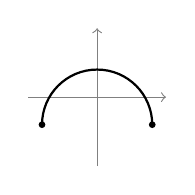
\begin{tikzpicture}[scale=0.35]
			% axes
			\draw[->,black!50] (-2.5, 0) -- (2.5, 0);
			\draw[->,black!50] (0, -2.5) -- (0, 2.5);
			% hemisphere
			\draw[thick] (-2, -1) arc (180:0:2);
			% end points
			\draw[fill] (-2, -1) circle (0.1);
			\draw[fill] ( 2, -1) circle (0.1);
		\end{tikzpicture}
		}
		\quad\xto{/{\sim}}\quad
		\centerbox{
		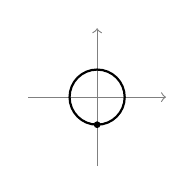
\begin{tikzpicture}[scale=0.35]
			% axes
			\draw[->,black!50] (-2.5, 0) -- (2.5, 0);
			\draw[->,black!50] (0, -2.5) -- (0, 2.5);
			% sphere
			\draw[thick] (0, 0) circle (1);
			% end points
			\draw[fill] (0, -1) circle (0.1);
		\end{tikzpicture}
		}
	\]
	\caption{Construction of the homeomorphism~$\disk^1 / {∼} ≅ \sphere^1$.}
	\label{construction of disk modulo sphere}
\end{figure}

We regard~$ℝ^{n + 1}$ as~$ℝ^n × ℝ$, writing elements of~$ℝ^{n + 1}$ as pairs~$(x, h)$ with~$x ∈ ℝ^n$ and~$h ∈ ℝ$.
We consider the hemisphere
\[
	H ≔ \{ (x, h) ∈ ℝ^{n + 1} \suchthat h ∈ [0, 1], \norm{x}^2 + h^2 = 1 \} \,.
\]
The hemisphere~$H$ is homeomorphic to the disk~$\disk^n$ via the mutually inverse continuous maps
\[
	\disk^n \to H \,, \quad x \mapsto (x, \sqrt{1 - \norm{x}^2}) \,,
\]
and
\[
	H \to \disk^n \,, \quad (x, h) \mapsto x \,.
\]
The equivalence relation~$∼$ on~$\disk^n ⊆ ℝ^n × ℝ$ corresponds to the equivalence relation~$∼$ on~$C$ that identifies all points in~$\sphere^{n - 1} × \{ 0 \}$, i.e., all points~$(x, h)$ in~$C$ with~$h = 0$.

The hemisphere~$H$ contains only points~$(x, h)$ with~$h ∈ [0, 1]$, whereas the sphere~$\sphere^n$ contains point~$(x, h)$ with~$h ∈ [-1, 1]$.
We now scale and translate the hemisphere~$H$ so that the resulting larger hemisphere~$H'$ contains points~$(x, h)$ with~$h ∈ [-1, 1]$ instead.
We consider therefore
\[
	H' = \{ (x, h) ∈ ℝ^{n + 1} \suchthat h ∈ [-1, 1], \norm{x}^2 + (h + 1)^2 = 4 \} \,,
\]
which is the upper hemisphere of the sphere with radius~$2$ and center~$(0, -1)$.
The hemispheres~$H$ and~$H'$ are homeomorphic via the mutually inverse continuous maps
\[
	H \to H' \,, \quad y \mapsto 2 y - (0, 1)
\]
and
\[
	H' \to H \,, \quad z \mapsto \frac{z + (0, 1)}{2} \,.
\]
The equivalence relation~$∼$ on~$H$ corresponds to the equivalence relation~$∼$ on~$H' ⊆ ℝ^n × ℝ$ that identifies all points in~$(2\sphere^{n - 1}) × \{ -1 \}$, i.e., all points~$(x, h)$ in~$H'$ with~$h = -1$.

We consider finally the map
\[
	f
	\colon
	H' \to \sphere^n \,,
	\quad
	(x, h) \mapsto (λ(h) x, h)
\]
where the scalar~$λ(h)$ is given by
\begin{align*}
	λ(x)
	= \frac{\sqrt{1 - h^2}}{\norm{x}}
	= \frac{\sqrt{1 - h^2}}{\sqrt{4 - (h + 1)^2}}
	= \sqrt{ \frac{1 - h^2}{3 - 2h - h^2} }
	&= \sqrt{ \frac{(1 + h)(1 - h)}{(3 + h)(1 - h)} } \\
	&= \sqrt{ \frac{1 + h}{3 + h} } \,.
\end{align*}
The map~$λ \colon H' \to ℝ$ is continuous, therefore~$f$ is continuous.

For every height~$h ∈ [-1, 1]$, the intersection of~$H'$ with the plane~$ℝ^n × \{ x \}$ is a circle with radius~$\sqrt{4 - (h + 1)^2}$, and the map~$f$ rescales this circle to have radius~$\sqrt{1 - h^2}$ instead.
We find that~$f$ maps the points~$(x, h)$ of~$H'$ with~$h ∈ (-1, 1]$ bijectively onto the punctured sphere~$\sphere^n ∖ \{ (0, -1) \}$, and all points~$(x, h)$ with~$h = -1$ onto the single point~$(0, -1)$ of~$\sphere^n$.
Consequently,~$f$ descends to a bijection~$g$ from~$H' / {∼}$ to~$\sphere^n$.
By the universal property of the quotient topology, this induced bijection~$g$ is again continuous.

To see that~$g$ is already a homeomorphism, we employ Corollary~2.18.2:
the disk~$\disk^n$ is compact and the sphere~$\sphere^n$ is a Hausdorff space, hence~$f$ is an embedding.
The induced continuous bijection~$g$ is therefore a homeomorphism.

We have overall constructed homeomorphisms
\[
	\disk^n / {∼} ≅ H / {∼} ≅ H' / {∼} ≅ \sphere^n \,.
\]
